\subsection{Runtime Adaptation}
\label{sec:runtime}

At runtime, \sysname{} performs application adaptation according to the learned
profile. We choose to design our own runtime system and adaptation algorithm
because prior solutions are not satisfactory: $(i)$~network protocols adapt to
available resources without application accuracy guarantee; $(ii)$
JetStream~\cite{rabkin2014aggregation} uses manual policies without the
bandwidth demand of each rule, therefore it can only react slowly and adapt
gradually, causing high latency; and $(iii)$~video streaming adaptation, such as
Huang et al.~\cite{huang2014buffer}, relies on the playback buffer and incurs
high latency.

Our runtime differs from prior systems in the ability to react
with precision: it stays in a low-latency state and uses a Pareto-optimal
configuration for high accuracy.

\begin{figure}
  \centering
  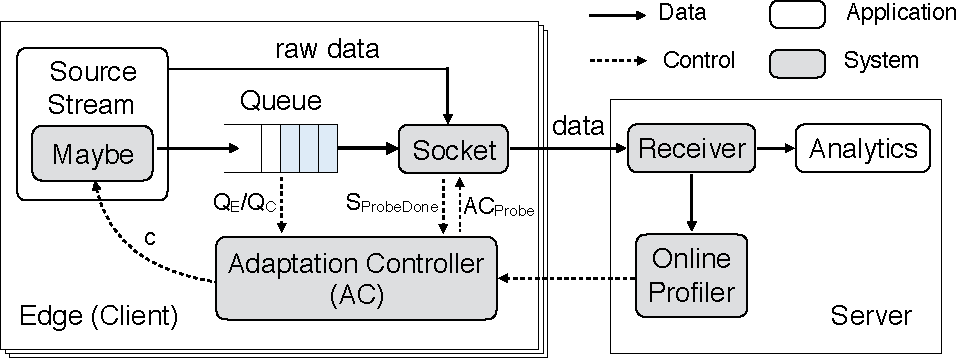
\includegraphics[width=\linewidth]{figures/runtime-adaptation.pdf}
  \caption{Runtime adaptation system architecture.}
  \label{fig:runtime}
\end{figure}

\autoref{fig:runtime} shows our runtime system architecture. \sysname{}
applications' source contains a \texttt{Maybe} module derived from all \maybe{}
operations. This module allows the controller to update the level of
degradation. Data generated by the source is then enqueued to \texttt{Queue} and
subsequently dequeued by \texttt{Socket}. When the data generation rate exceeds
\texttt{Socket}'s departure rate, the queue grows. In this case, the adaptation
controller (AC) queries the estimated bandwidth from \texttt{Socket} and
regulates the source stream by updating the configuration.  After the data is
sent through the network, the receiver extracts raw data to the online profiler
and delivers data to the application analytics. Raw data is only transmitted
when the queue is empty. When a new profile is learned, it is fed back to AC for
subsequent adaptation.

We then describe the adaptation algorithm; \autoref{fig:cc} shows the state machine model and an example trace for illustration.
AC loads the profile and sorts all configurations with an
ascending order of bandwidth demand, resulting in a list $[c_1, \dots,
c_{\max}]$.
These configurations follow a total order: $c_i < c_j$ if $B(c_i) < B(c_j)$.
We denote the current configuration as $c_i$ and the next $c_{i+1}$.
AC receives messages from the \texttt{Queue}: message \qe{} when the queue is empty
and $\text{Q}_\text{C}$ when queued items exceed a threshold. AC can query
\texttt{Socket} for delivery rate $R$ or request it to probe ($\text{AC}_{\text{Probe}}$) for a target
bandwidth, often $B(c_{i+1})$. When $R > B(c_{i+1})$, \texttt{Socket} sends back
\spd{}. The algorithm follows a state machine as described below:

\begin{itemize}[leftmargin=*, topsep=3pt, itemsep=0pt]

\item \textbf{Startup: rapid growth.} \sysname{} starts with $c_1$ and grows the
  rate ($c_i \Rightarrow c_{i+1}$) upon each \qe{}. The growth stops at
  $c_{\max}$ (to \texttt{Steady}) or if it receives \qc{} (to \texttt{Degrade}).

\item \textbf{Degrade: reacting to congestion.} When \texttt{Queue} grows and
  exceeds a threshold, AC receives \qc{} and runs the \texttt{adapt()}
  procedure. This involves two steps: (1) AC queries $R$ from \texttt{Socket};
  (2) AC updates \texttt{Maybe} with the maximum-allowed $c$ that satisfies
  $B(c) < \alpha R, \alpha \in (0, 1)$. A smaller $\alpha$ allows a quicker
  draining of the queue. After the queue is drained, \sysname{} changes to
  \texttt{Steady}.

\item \textbf{Steady: low latency delivery.} \sysname{} achieves low latency by
  spending most of the time in the \texttt{Steady} state. It changes to
  \texttt{Degrade} when congestion occurs. If $c < c_{\max}$ and it receives
  \qe{}, AC enters the \texttt{Probe} state to check for more available
  bandwidth.

\item \textbf{Probe: more bandwidth for a higher accuracy.} Advancing the configuration
  directly causes a drastic latency increase when $B(c_{i+1}) \gg B(c_i)$. To
  allow a smooth increase, AC requests \texttt{Socket} to probe by sending
  additional traffic controlled by \texttt{probe\_gain} (in
  \texttt{inc\_pace()}, similar to BBR~\cite{cardwell2017bbr}). \sysname{} stops
  probing under two conditions: (1) upon \spd{}, it advances $c_i$; (2) upon
  \qc{}, it returns to \texttt{Steady}.

\end{itemize}

\begin{figure}
  \begin{subfigure}[t]{\columnwidth}
    \centering
    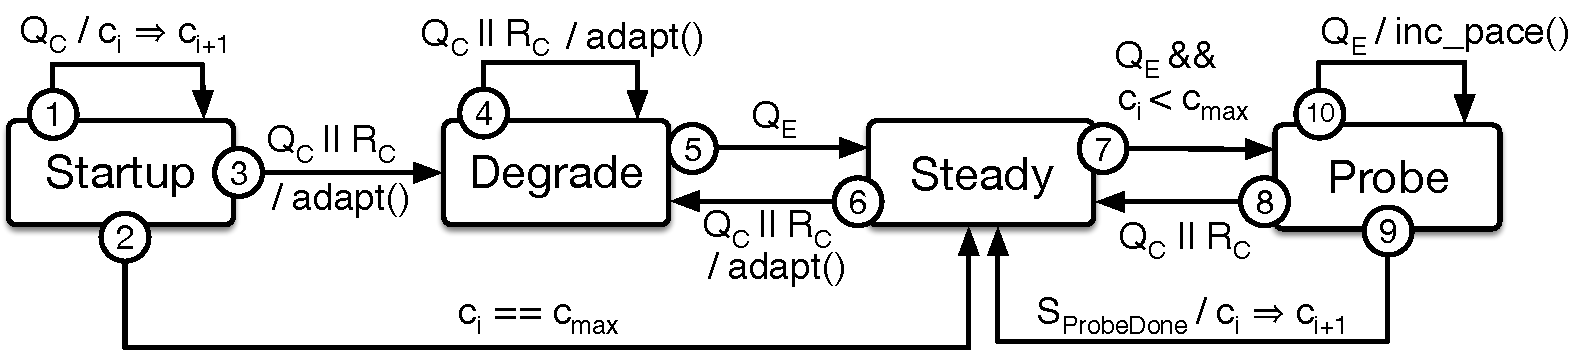
\includegraphics[width=\columnwidth]{figures/cc.pdf}
    \caption{Rate adaptation as a state machine.}
    \vspace{1em}
    \label{fig:cc-sm}
  \end{subfigure}
  \begin{subfigure}[t]{\columnwidth}
    \centering
    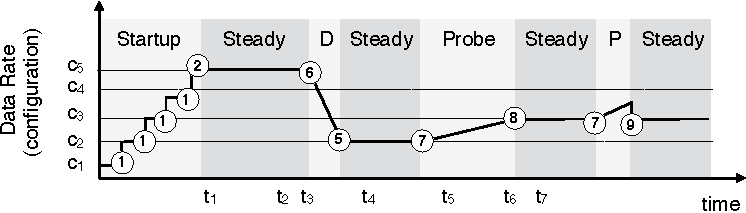
\includegraphics[width=\columnwidth]{figures/cc2.pdf}
    \caption{An example illustrating the adaptation algorithm.}
    \label{fig:cc-ex}
  \end{subfigure}
  \caption{Runtime adaptation algorithm.}
  \label{fig:cc}
\end{figure}

% \begin{figure}
%   \centering
%   \resizebox{\columnwidth}{!}{
%     \begin{tikzpicture}[
  state/.style = { draw, very thick, fill=white, rounded corners=1em,
    minimum height=3em, minimum width=7em, node distance=7em, font={\bfseries},
    align=center },
  edge portion/.style = { black, thick },
  transition/.style = { edge portion, -> },
  algorithm/.style = { draw, thin, fill=white },
  ]

  \node [state] (startup) {
    STARTUP };
  \node [state] (congestion) [right=of startup] {CONGESTION};
  \draw [transition] (startup) -- (congestion)
  node [midway, auto] {Q.Congestion};

  \node [state] (steady) [below=of congestion] {STEADY};

  \draw [transition] ($(congestion.south west)!0.4!(congestion.south east)$)
  to node[midway, sloped, below] {Q.NoQueue}
  ($(steady.north west)!0.4!(steady.north east)$);

  \draw [transition] ($(steady.north west)!0.6!(steady.north east)$)
  to node[midway, sloped, below] {Q.Congestion}
  ($(congestion.south west)!0.6!(congestion.south east)$);

  \node [state] (probe) [left=of steady] {PROBE};

  \draw [transition] ($(steady.south west)!0.6!(steady.north west)$)
  -- ($(probe.south east)!0.6!(probe.north east)$)
  node[midway, auto, swap] {Q.Probe};

  \draw [transition, <-] ($(steady.south west)!0.4!(steady.north west)$)
  -- ($(probe.south east)!0.4!(probe.north east)$)
  node[midway, auto, align=left] {Q.Congestion | \\ IO.ProbeDone};

\end{tikzpicture}


%%% Local Variables:
%%% mode: latex
%%% TeX-master: "sosp17"
%%% End:

%   }
%   \caption{Congestion Control Algorithm}
%   \label{fig:cc}
% \end{figure}

\para{Resource Allocation and Fairness.} In addition to rate adaptation, the
profile is also useful for controlling a single application's bandwidth usage or allocating resources among competing tasks.

For individual applications, developers can pinpoint a configuration for a given
bandwidth or accuracy goal. They can also specify a criterion to limit effective
configurations. For example, \sysname{} can enforce an upper bound on the
bandwidth consumption, useful to reduce WAN bandwidth usage and cost.

For multiple applications, their profiles allows novel bandwidth allocation
schemes such as utility fairness. Different from traditional resource fairness
where applications get equal share of bandwidth, utility fairness aims
to maximize the \textit{minimal} application accuracy. With the profiles,
finding allocations is equivalent to finding proper configuration $c^t$ for
application $t$. We formulate utility fairness as follows:

%% Pick one based on the space

%\begin{equation}
 % \label{eq:multitask}
%  \underset{c^t}{\max} \; \min({A^t(c^t)})
%  \;
%  \text{s.t.}
%%  \;
%%  \sum_t{B^t(c^t)} < R
%% \end{equation}

\begin{equation}
 \label{eq:multitask}
 \begin{aligned}
    & \underset{c^t}{\text{maximize}} & & \min({A^t(c^t)}) & & \\
    & \text{subject to} & & \sum_t{B^t(c^t)} < R & & \\
 \end{aligned}
\end{equation}

Solving this optimization is computationally hard. \sysname{} uses a heuristics
approach. We start with $c_1^t$ and improve the application $t$ that has the
worst accuracy. This process repeats until we have allocated all available
bandwidth.

%%% Local Variables:
%%% mode: latex
%%% TeX-master: "awstream"
%%% End:
